\documentclass{standalone}

\usepackage{tikz}
\usetikzlibrary{automata, arrows.meta, positioning, shapes}

\begin{document}
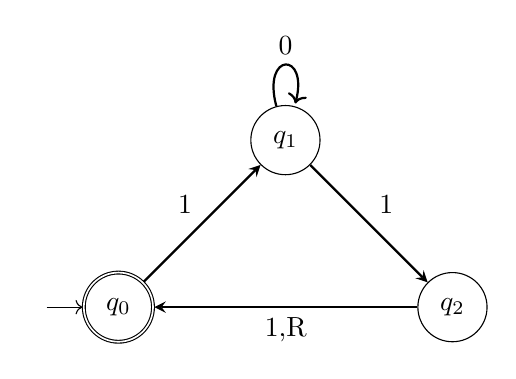
\begin{tikzpicture} [node distance = 3 cm, on grid, auto]
  \node (q0) [state, initial, accepting, initial text = {}] {$q_{0}$};
  \node (q1) [state, above right = of q0] {$q_{1}$};
  \node (q2) [state, below right = of q1] {$q_{2}$};
  \path [-stealth, thick]
    % (q0) edge [above] node {1} (q1)
    (q0) edge node {1} (q1)
    (q1) edge node {1} (q2)
    %(q1) edge [loop] node {0} ();
    (q1) edge [loop above] node {0} ()
    (q2) edge node {1,R} (q0);
\end{tikzpicture}
\end{document}
